%%% Copyright (C) 2018 Vincent Goulet
%%%
%%% Ce fichier fait partie du projet
%%% «Programmer avec R»
%%% https://gitlab.com/vigou3/programmer-avec-r
%%%
%%% Cette création est mise à disposition selon le contrat
%%% Attribution-Partage dans les mêmes conditions 4.0
%%% International de Creative Commons.
%%% https://creativecommons.org/licenses/by-sa/4.0/

\chapter{Travail collaboratif avec Git}
\label{chap:git}

\begin{objectifs}
\item Créer une version locale d'un projet informatique hébergé dans
  un dépôt utilisant le système de gestion de version Git.
\item Créer, utiliser et supprimer une branche dans un projet avec
  Git.
\item Publier des ajouts et des modifications à un projet avec Git.
\item Rendre disponibles des ajouts et des modifications à une
  communauté par le biais d'un serveur Git.
\end{objectifs}

Nous avons déjà traité, à la \autoref{sec:fonctions:pratiques} de
bonnes pratiques à adopter en matière de style de programmation et de
présentation du code dans un contexte de travail collaboratif. Un
autre enjeu surgit toutefois dès que plus d'une personne œuvre sur un
projet: le partage et l'échange des contributions de chacun. Comment
rendre le travail de Marianne disponible à Alexandre? Comment
s'assurer qu'une modification apportée dans un fichier par Alexandre
n'écrase pas celle sur laquelle Marianne travaille depuis plusieurs
heures? Comment identifier à coup sûr et automatiquement la plus
récente version d'un fichier? Ce genre de questions, auxquelles
quiconque a déjà travaillé en équipe sur un projet a déjà été
confronté, les informaticiens y ont répondu depuis de très nombreuses
années avec les systèmes de gestion de versions.

J'offre, dans ce chapitre, une courte introduction à ces outils de
développement incontournables avant de vous diriger vers la
documentation officielle du système de gestion le plus utilisé dans le
monde en ce moment: Git.


\section{Gestion des versions}
\label{sec:collaboration:git}

Un système de gestion de versions gère l'ensemble des versions --- ou
\emph{révisions} --- d'un ou plusieurs fichiers, normalement en format
texte. Dans le monde de la programmation, un tel système se charge du
maintient du code source d'un projet logiciel. Il enregistre la
nature, la date et l'auteur de chaque révision apportée à un fichier
et il permet ensuite de retourner à des révisions précédentes, de
comparer des révisions entre elles ou de fusionner des révisions.

Outil incontournable en contexte de travail collaboratif, le système
de gestion de version permet de régler les problèmes de suivi de la
plus récente version d'un fichier, de partage de fichiers entre les
membres d'une équipe et de mise en commun des contributions. Comme les
versions successives sont entreposées dans un référentiel situé sur un
serveur central, le système fournit également une forme de copie de
sauvegarde du code source d'un projet.

\tipbox{L'utilisation d'un système de gestion de versions vaut le coup
  même pour vos projets strictement individuels, ne serait-ce que pour
  les volets de copie de sauvegarde et de suivi des versions.}

Les systèmes de contrôle de version de première génération ont vu le
jour dans les années 1970 et 1980:
\link{https://fr.wikipedia.org/wiki/Source_Code_Control_System}{Source
    Code Control System} (SCCS, 1972),
\link{https://fr.wikipedia.org/wiki/GNU_RCS}{Revision Control
    System} (RCS, 1982). Ces systèmes ne permettaient pas de
travailler à plusieurs à la fois sur un même fichier. Cette barrière a
été levée par les systèmes centralisés de seconde génération qui ont
pu se développer grâce à l'accès de plus en plus généralisé à la
réseautique --- notamment à Internet --- au cours des années 1990 et
2000. Pendant plus d'une décennie, le système libre
\index{CVS}\link{https://fr.wikipedia.org/wiki/Concurrent_versions_system}{Concurrent
    Versions System} (CVS, 1990) a régné sur le monde de la gestion
de versions, jusqu'à l'arrivée de
\index{Subversion}\link{https://fr.wikipedia.org/wiki/Apache_Subversion}{Apache
    Subversion} (SVN, 2000). Construit selon les mêmes principes que
CVS et compatible avec lui, Subversion se voulait surtout une
meilleure implémentation d'un système de gestion de version
centralisé. Le système est rapidement devenu le standard \emph{de
  facto}, si bien que le code source de plusieurs projets
informatiques est toujours administré avec Subversion.

Par leur nature, les systèmes centralisés requièrent un accès au
serveur central pour toute opération de publication d'une modification
à un fichier. C'est pour lever cette contrainte que sont apparus, au
milieu des années 2000, les systèmes de gestion de version distribués.
Les principaux représentants de cette troisième génération de systèmes
sont \index{Git}\link{https://fr.wikipedia.org/wiki/Git}{Git} (2005),
\index{Mercurial}\link{https://fr.wikipedia.org/wiki/Mercurial}{Mercurial} (hg,
2005) et
\index{Bazaar}\link{https://fr.wikipedia.org/wiki/Bazaar_(logiciel)}{Bazaar}
(bzr, 2005).

\Index{Git}Git a été développé à l'origine par Linus Torvalds pour
administrer le code source du noyau du système d'exploitation Linux.
Le système a connu une popularité foudroyante, notamment grâce à
GitHub, un site d'hébergement de projets libres basé sur Git et doté
d'une interface particulièrement conviviale. Résultat: Git est
aujourd'hui le système de gestion de versions le plus utilisé dans le
monde.

Après cette entrée en matière, je vous renvois vers \emph{Pro Git}
\citep{ProGit:2e:2014}, qui fait partie de la documentation officielle
de Git, pour apprendre les rudiments du système. Cet l'ouvrage libre
est particulièrement bien fait. Pour atteindre les objectifs
d'apprentissage fixés en entête de chapitre, vous devez couvrir les
sections suivantes de \emph{Pro Git}:
\begin{itemize}
\item chapitre 1, toutes les sections, sauf la section~1.5 sur
  l'installation de Git;
\item chapitre 2, sections 2.1, 2.2 et 2.5 (les sections 2.3 et 2.4 sont
  optionnelles, mais utiles);
\item chapitre 3, sections 3.1, 3.2 et 3.3.
\end{itemize}
Pour votre commodité, ces sections sont reproduites à
l'\autoref{chap:git}.

Créez un compte dans l'un des nombreux dépôts Git publics
(\link{https://github.com}{GitHub}, \link{https://gitlab.com}{GitLab},
\link{bitbucket.org}{BitBucket}, pour ne nommer que ceux-là) et
commencez à vous familiariser avec le cycle de travail de Git pour un
projet personnel. Ajoutez ensuite graduellement le volet de %
\capsule{https://youtu.be/bdIjgjg6zoc}{travail collaboratif}. %

\begin{figure}[t]
  \begin{emphbox}{\mdseries Configuration de l'éditeur de texte pour
      les messages de Git}
    La \autoref{sec:git:first_time} mentionne la possibilité de
    configurer l'éditeur de texte qui sera utilisé quand Git doit vous
    demander de saisir un message. Dans le seul exemple qui est
    fourni, c'est Emacs qui est utilisé comme éditeur en remplacement
    de Vim.

    Il y a fort à parier que vous souhaiterez configurer Git pour
    utiliser un éditeur plus convivial.

    \begin{description}
    \item[Windows]
    Le plus simple sous Windows consiste à utiliser le Bloc-notes.
    Entrez la commande suivante à l'invite de commande (Git Bash) pour
    choisir cet éditeur par défaut:
    \begin{Schunk}
\begin{Verbatim}
$ git config --global core.editor notepad
\end{Verbatim}
    \end{Schunk}%$

    \item[macOS]
    Le meilleur truc sous macOS consiste à utiliser la commande
    générique \code{open} pour ouvrir un fichier. Ainsi, c'est votre
    éditeur de fichiers par défaut du Finder qui sera utilisé à tout
    coup. Par défaut, il s'agit de TextEdit. Entrez la commande
    suivante à l'invite de commande du Terminal:
    \begin{Schunk}
\begin{Verbatim}
$ git config --global core.editor open
\end{Verbatim}
    \end{Schunk}
  \end{description}

    \emph{Sources}:
    \link{https://stackoverflow.com/questions/10564/how-can-i-set-up-an-editor-to-work-with-git-on-windows}{How
      can I set up an editor to work with Git on Windows?},
    \link{https://stackoverflow.com/questions/3539594/change-the-default-editor-for-files-opened-in-the-terminal-e-g-set-it-to-text}{Change the default editor for files opened in the terminal?}
  \end{emphbox}
  \label{fig:colloration:editeur}
\end{figure}


\section{Exemples}
\label{sec:collaboration:exemples}

\def\scriptfilename{collaboration.R}

\scriptfile{\scriptfilename}
\lstinputlisting[firstline=\scriptfirstline]{\scriptfilename}


\section{Exercices}
\label{sec:collaboration:exercices}

\Opensolutionfile{solutions}[solutions-collaboration]

\begin{Filesave}{solutions}
\section*{Chapitre \ref*{chap:collaboration}}
\addcontentsline{toc}{section}{Chapitre \protect\ref*{chap:collaboration}}

\end{Filesave}

\begin{exercice}[nosol]
  Configurer votre éditeur de texte pour indenter le code R de quatre
  (4) caractères. Dans RStudio, ouvrir le panneau des options
  globales, sélectionner la catégorie \code{Code} et inscrire la
  valeur \code{4} dans le champs \code{Tab width} (voir la
  \autoref{fig:collaboration:rstudio-tab-width}).
  \begin{figure}
    \centering
    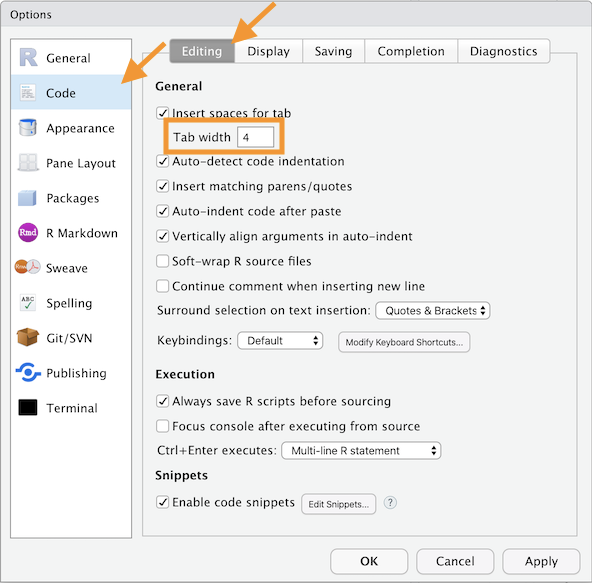
\includegraphics{images/rstudio-tab-width}
    \caption{Configuration de RStudio pour indenter le code de quatre
      caractères}
    \label{fig:collaboration:rstudio-tab-width}
  \end{figure}
\end{exercice}

\begin{exercice}[nosol]
  Configurer l'éditeur par défaut de Git sur votre poste de travail
  tel qu'expliqué dans l'encadré de la
  \autopageref{fig:colloration:editeur}.
\end{exercice}

\begin{exercice}
  Présenter le code ci-dessous selon les normes d'espacement,
  d'indentation et de positionnement des accolades mentionnées à la
  \autoref{sec:collaboration:presentation}. Pour ajuster
  automatiquement l'indentation avec RStudio, sélectionner le bloc de
  code et choisir dans les menus \code{Code|Reformat Code}.

\begin{Schunk}
\begin{Verbatim}
f <- function(x){
  if(all(x>=0)|| all(x<=0))
  { stop("all x are the same sign")
  }
  if (sum(diff(sign(x[x!=0]))!=0)>1)
  warning("more than one sign change")
 r<-polyroot(x)
i<-1/Re(r)[abs(Im(r))< .Machine$double.eps^0.5]-1
i[i > -1]
}
\end{Verbatim}
\end{Schunk}
\begin{sol}
  La présentation correcte comporte des espaces autour de tous les
  opérateurs, une indentation de quatre (4) caractères et des
  accolades ouvrante et fermante placées sur leur propre ligne.
\begin{Schunk}
\begin{Verbatim}[fontsize=\relsize{-1}]
tri <- function(x)
{
    if (all(x >= 0) || all(x <= 0))
    {
        stop("all x are the same sign")
    }
    if (sum(diff(sign(x[x != 0])) != 0) > 1)
        warning("more than one sign change")
    r <- polyroot(x)
    i <- 1/Re(r)[abs(Im(r)) < .Machine$double.eps^0.5] - 1
    i[i > -1]
}
\end{Verbatim}
\end{Schunk}
\end{sol}
\end{exercice}

\begin{exercice}[nosol]
  Suivre le tutoriel interactif \link{https://try.github.io/}{tryGit}
  pour vous familiariser avec les commandes principales de Git.
\end{exercice}

\begin{exercice}
  Créer un compte chez \link{https://github.com}{GitHub}, puis créer
  un «embranchement» (\emph{fork}) du projet test
  \link{https://github.com/octocat/Spoon-Knife}{Spoon-Knife} depuis
  l'interface graphique de GitHub. Vous disposerez alors d'une copie
  de ce projet dans vos propres projets. Effectuer ensuite les
  opérations suivantes.
  \begin{enumerate}
  \item Cloner le projet sur votre poste de travail.
  \item Créer une branche locale pour effectuer une modification au
    projet.
  \item Modifier le fichier \code{index.html} d'une manière
    quelconque.
  \item Publier localement la modification dans la branche.
  \item Publier la branche dans le dépôt GitHub.
  \item Effectuer une «demande de tirage» (\emph{pull request}) dans
    le projet original à partir de l'interface de GitHub. Comme il
    s'agit d'un dépôt test, elle sera ignorée.
  \end{enumerate}

  \begin{sol}
    Pour créer l'embranchement (\emph{fork}), il suffit d'appuyer sur
    le bouton \code{Fork} en haut à droite de la page
    \link{https://github.com/octocat/Spoon-Knife}{Spoon-Knife}.
    Ensuite, les commandes à exécuter depuis une ligne de commande
    \index{Git~Bash}Git~Bash (Windows) ou \index{Terminal}Terminal
    (macOS) sont les suivantes, dans l'ordre:
\begin{Schunk}
\begin{Verbatim}[commandchars=\\\{\},fontsize=\relsize{-1}]
~$ git clone https://github.com/\meta{username}/Spoon-Knife.git
~$ cd Spoon-Knife
~/Spoon-Knife$ git checkout -b \meta{nom_branche}
\meta{modifier le fichier index.html avec son éditeur}
~/Spoon-Knife$ git status
~/Spoon-Knife$ git add index.html
~/Spoon-Knife$ git commit -m "\meta{message}"
~/Spoon-Knife$ git push -u origin \meta{nom_branche}
\end{Verbatim}
\end{Schunk}
    Enfin, retourner sur la page du projet d'origine et appuyer sur le
    bouton \code{Compare \& pull request} et suivre les instructions.
    Votre demande de tirage devrait ensuite apparaitre dans la liste
    de toutes les demandes du projet (plus de \nombre{5000} au moment
    d'écrire ces lignes).
  \end{sol}
\end{exercice}

\Closesolutionfile{solutions}


%%% Local Variables:
%%% mode: latex
%%% TeX-engine: xetex
%%% TeX-master: "programmer-avec-r"
%%% coding: utf-8
%%% End:
,,